% !TEX root = main.tex

\subsection{Parameter Sensitive}

\begin{figure}[!]
    \centering
    % \vspace{-0.2em}
    \begin{subfigure}[]{0.23\textwidth}
        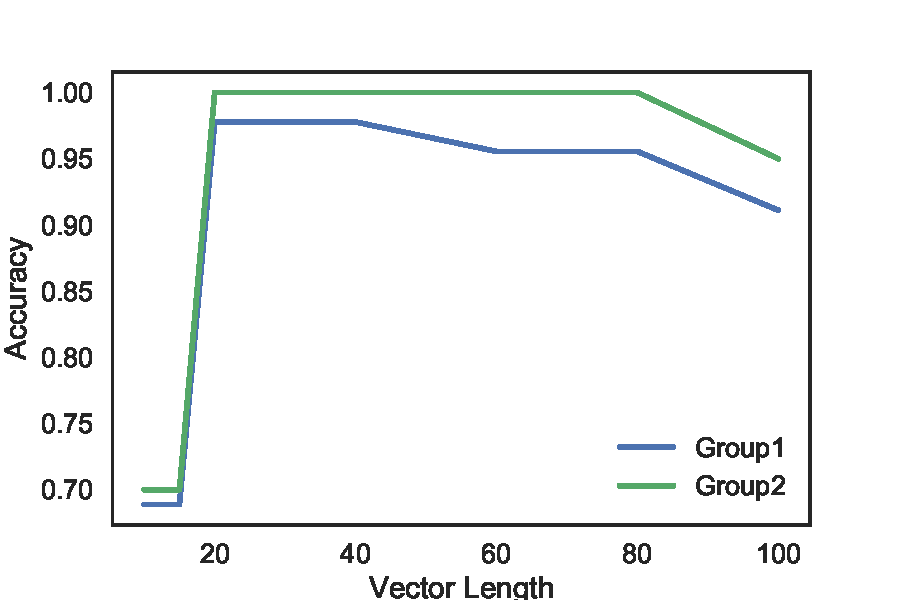
\includegraphics[width=\textwidth]{img/curve3.pdf}
        \caption{Fitting Observed Facts}
        \label{fig:sensitive-best-accuracy-1}
        %\vspace{-0.3em}
    \end{subfigure}
    \begin{subfigure}[]{0.23\textwidth}
        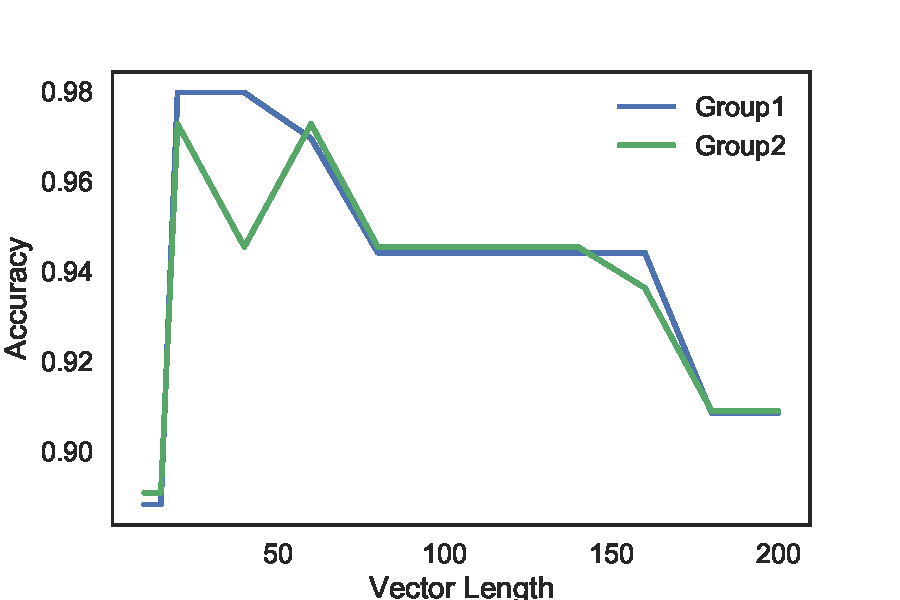
\includegraphics[width=\textwidth]{img/curve4.pdf}
        \caption{Learning from Rules }
        \label{fig:sensitive-best-accuracy-2}
        %\vspace{-0.3em}
    \end{subfigure}
    \caption{Best Accuracy w.r.t. Vector Length.}
    \label{fig:sensitive}
    % \vspace{-1.2em}
\end{figure}


In this part, we want to test the effect of vector length $k$. We enumerate the vector length from 1 to 100 and shows the best accuracy on two groups. We did our experiments on both observed data and weighted dataset with rule. As the performance of C-LNT is better than LNT, we only shows the result of C-LNT, which is shown in Figure \ref{fig:sensitive}.

Figure \ref{fig:fitting-best-accuracy-1} shows the result in observed dataset.
From this figure, we can conclude that the performance is not always getting better with the increase of vector length. Actually, it's getting worse when $k$ is too big. That's may because the under training problem. That is, as we increase the vector length, we may need to repeat more to get a good model. Those effors is unnecessary because we would get a good result when $k \in [20,40]$.
